% Illustration and advantages of variable capacity
\begin{slide}[Les PàCCV adaptent leur capacité aux besoins\\
			  pour fonctionner de façon continue]

% Illustration
\only<1>{
\node[anchor=mid west, align=left] at (p5cl cs:1,11) {capacité\\fixe};
\node[anchor=mid west, align=left] at (p5cl cs:1,3) {capacité\\variable};

\begin{scope}[shift={(p5cr cs:1,10)},
			  x=\bigcol/6+\baselineskip/6, y=3\baselineskip]

\draw[semithick] (0,.3333333) -- (3,.33333333) |- (6,.666666);
\draw[col, very thick]
	  (0,0) .. controls (0.1, 1) and (0.2, 1) .. (0.5,1)
   -- (0.5,1) .. controls (0.52, 0) and (0.6, 0) .. (0.7,0)
   -- (1.5,0) .. controls (1.6, 1) and (1.7, 1) .. (2,1)
   -- (2,1) .. controls (2.02, 0) and (2.1, 0) .. (2.2,0)
   -- (3,0) .. controls (3.1, 1) and (3.2, 1) .. (3.5,1)
   -- (4,1) .. controls (4.02, 0) and (4.1, 0) .. (4.2,0)
   -- (4.5,0) .. controls (4.6, 1) and (4.7, 1) .. (5,1)
   -- (5.5,1) .. controls (5.52, 0) and (5.6, 0) .. (5.7,0) -- (6,0);
	
\end{scope}


\node[becomes, rotate=180] at (p5cr cs:2,7.5) {};


\begin{scope}[shift={(p5cr cs:1,2)},
			  x=\bigcol/6+\baselineskip/6, y=\baselineskip]

\draw[semithick] (0,1) -- (3,1) |- (6,2);
\def\phase{46.87329}  % found numerically with scipy
\draw[col, very thick] plot[domain=0:3, samples=100, smooth]
			(\x, {1 - exp(-2*\x) * cos(700*\x + \phase) / cos(\phase)});
	
\end{scope}


\begin{scope}[shift={($(p5cr cs:1,3)+(\colv+\baselineskip,0)$)},
			  x=\bigcol/6+\baselineskip/6, y=\baselineskip]

% use rect line cap for joining but clip the part sticking out
\clip (p5cr cs:1,3) rectangle ++(2\colvsep,3\baselineskip);
\def\phase{46.87329}
\draw[col, very thick, line cap=rect] plot[domain=0:3, samples=100, smooth]
			(\x, {1 - exp(-2*\x) * cos(700*\x + \phase) / cos(\phase)});
\end{scope}
}


% Advantages
\only<2->{
\node[anchor=base west, align=left] (list) at (t5cr cs:1,5){
	\begin{minipage}[b]{2\colvsep}
	\hskip-.8pt Et ainsi augmentent\\
	\begin{listed}
        \item la performance
        \item la plage de températures
    \end{listed}
    \end{minipage}};
}

\end{slide}



\begin{slide}[Un modèle dynamique adéquat est nécessaire\\
			  pour simuler correctement les PàCCV]

\node[anchor=base west] (text) at (t5cl cs:0,4) {
	\begin{minipage}[b]{\dimexpr2\colvsep+4\quanta}\raggedright
		\emph{Exemple}\\[2\baselineskip]
		Profil de consommation\\d'une unité de résidence typique,\\~\\
		avec un pas de temp $ \Delta t = \SI{1}{\minute} $
	\end{minipage}};

\node[anchor=south east] at (p5cr cs:4,3)
	{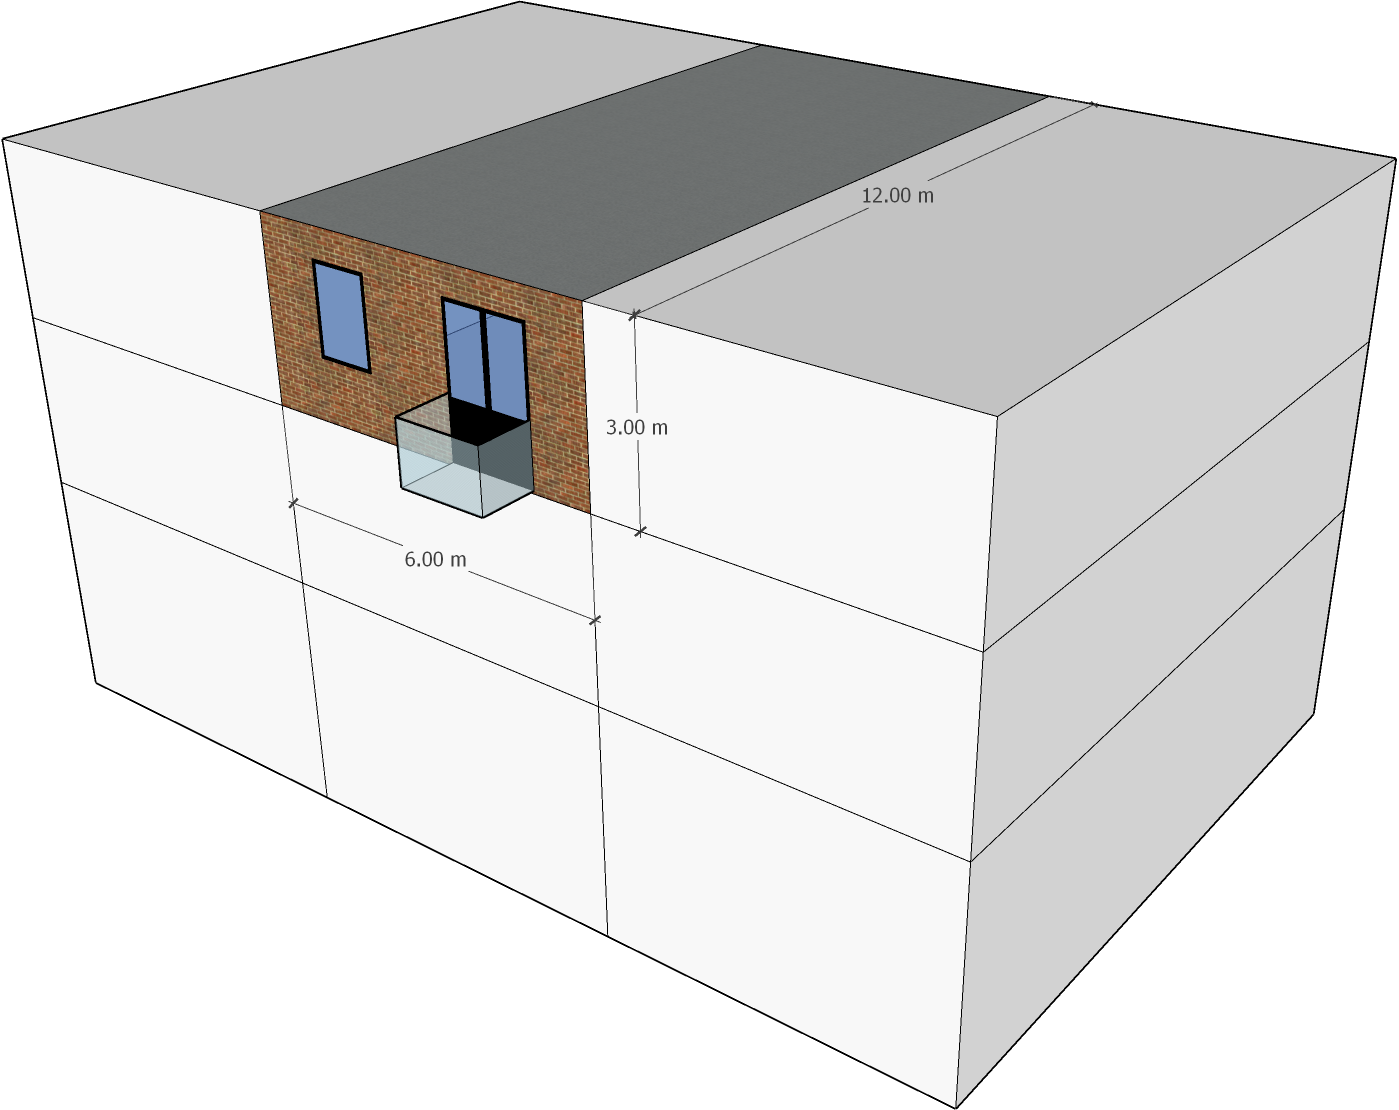
\includegraphics[height=9\baselineskip]{pictures/plex-unit}};

\end{slide}


% Données incomplètes
\begin{slide}[Les données des manufacturiers\\
			  sont généralement incomplètes]

\only<1>{
\begin{axis}[plot options, clip=false,
			 at={(p5cl cs:2,2)},
			 width=\bigcol+2\baselineskip, height=12\baselineskip,
			 xtick={-26.1, 15},
			 xticklabels={\num{-26.1}\phantom{$-$}, \SI{15}{\celsius}},
			 ytick={1.42, 4.75},]
\foreach \i in {1, ..., 4}{
	\addplot[mark=*, mark size=1pt, semithick] table[x=Toa, y=COP_at_T\i]
		{data/manu-data-heating.tsv};}
\foreach \i/\COP in {1/4.75, 2/4.524, 3/4.339, 4/3.961}{%
	\edef\temp{\noexpand\node (T\i) at (axis cs:15,\COP) {};}
	\temp}
\end{axis}
\node[anchor=mid west, font=\footnotesize] at (p5cl cs:1,14) {COP};
\node[anchor=base east, font=\footnotesize] (Toa)
	at (t5cr cs:4,0) {$ T_\text{oa} $};
\foreach \i/\Ti in {1/15.6, 2/18.3, 3/21.1, 4/23.8}{
	\node[font=\footnotesize, gray, anchor=east] (Tr\i)
		at (T\i -| Toa.east) {\SI{\Ti}{\celsius}};
	\draw[gray] (T\i)++(4.5pt,0) -- ($(Tr\i.west)-(4pt,0)$);}
\node[anchor=west, yshift=-2\baselineskip, font=\footnotesize]
	at (Tr4.west) {$T_r$};
}

\def\displayat{2}
\foreach \row/\rowlabel in {0/$f_3$, 1/$f_2$, 2/$f_1$}{
	\foreach \col/\collabel in {2/$\dot V_1$, 3/$\dot V_2$, 4/$\dot V_3$}{
		\colorlet{background}{gray!10}
		\ifnum \row=2
			\ifnum \col=2
				\temporal<3>{
					\colorlet{background}{gray!10}}{
					\colorlet{background}{gray!10}}{
					\colorlet{background}{col!20}}
			\fi
		\fi
		\ifnum \col=2
			\renewcommand\displayat{2}
		\else
			\renewcommand\displayat{3}
		\fi
		\begin{axis}[visible on=<\displayat->,
					 enlargelimits=false, scale only axis,
					 hide axis,
					 at={($(p5cl cs:\col,0)+(0,56*\row*\quantum/3)$)},
					 width=\colv, height=11\baselineskip/3,
					 axis background/.style={fill=background}]
		
		\foreach \i in {1, ..., 4}{
			\addplot[mark=*, mark size=.5pt] table[x=Toa, y=COP_at_T\i]
				{data/manu-data-heating.tsv};}
			
		\end{axis}
		\ifnum \row=0
			\node[xshift=.5\colv, anchor=base, visible on=<3->]
				at (p5cl cs:\col,14){\collabel};
		\fi
	}
	\pgfmathparse{2+\row}\let\labelypos\pgfmathresult
	\node[anchor=east, visible on=<2->] (row\row)
		at ($(p5cr cs:1,0)+(0,{(22+56*\row)*\quantum/3})$) {\rowlabel};
}

\node[anchor=base] (pct) at ($(t5cl cs:0,6)!0.5!(row1.base west)$)
	{$ {\uncover<4->{{\color{col}1}\above 0.4pt} \uncover<3->{3 \times 3}}
	   \uncover<4->{\approx \SI{11}{\percent}} $};

\uncover<3->{
	\node[align=left, font=\footnotesize] (required)
		at (pct.202 |- row0) {paires $ (f, \dot V) $\\nécessaires};
	\draw (pct.202)++(0,-4pt) -- ($(required.north)+(0,4pt)$);}
\uncover<4->{
	\node[align=left, font=\footnotesize] (provided)
		at (pct.158 |- row2) {paire $ (f, \dot V) $\\fournie};
	\draw[col] (pct.158)++(0,4pt) -- ($(provided.south)-(0,4pt)$);}		

\end{slide}
